% ============================================================================
% Ethereum, Smart Contracts & Stablecoins - Training Presentation
% AP3 Labs | 30-minute session
% Compile with: xelatex ethereum-training.tex (run twice for notes)
% ============================================================================

\documentclass[aspectratio=169, 11pt]{beamer}

% --- Packages ---------------------------------------------------------------
\usepackage{fontspec}
\usepackage{tikz}
\usepackage{graphicx}
\usepackage{hyperref}
\usepackage{setspace}
\usepackage{amssymb}

% --- Satoshi Font (from static/fonts/) --------------------------------------
\setsansfont{Satoshi}[
  Path           = static/fonts/,
  Extension      = .otf,
  UprightFont    = *-Regular,
  BoldFont       = *-Bold,
  ItalicFont     = *-Italic,
  BoldItalicFont = *-BoldItalic,
]
\setmainfont{Satoshi}[
  Path           = static/fonts/,
  Extension      = .otf,
  UprightFont    = *-Regular,
  BoldFont       = *-Bold,
  ItalicFont     = *-Italic,
  BoldItalicFont = *-BoldItalic,
]

\usetikzlibrary{
  arrows.meta,
  positioning,
  shapes.geometric,
  calc,
  fit,
  backgrounds,
  decorations.pathreplacing
}

% --- AP3 Labs Color Palette -------------------------------------------------
\definecolor{ap3dark}{HTML}{171717}
\definecolor{ap3light}{HTML}{CCD6F6}
\definecolor{ap3cream}{HTML}{FEFFFF}
\definecolor{ap3orange}{HTML}{FFA33C}
\definecolor{ap3slate}{HTML}{64748B}
\definecolor{ap3orange10}{HTML}{2D2317}    % orange tint on dark bg
\definecolor{ap3darkgray}{HTML}{222222}
\definecolor{ap3midgray}{HTML}{333333}

% --- Beamer Theme Configuration (Minimalist) --------------------------------
\usetheme{default}
\usecolortheme{default}

% Remove all navigation
\setbeamertemplate{navigation symbols}{}
\setbeamertemplate{footline}{}

% Backgrounds
\setbeamercolor{background canvas}{bg=ap3dark}
\setbeamercolor{normal text}{fg=ap3light}

% Titles
\setbeamercolor{frametitle}{fg=ap3cream}
\setbeamerfont{frametitle}{size=\Large, series=\bfseries}
\setbeamercolor{title}{fg=ap3orange}
\setbeamerfont{title}{size=\huge, series=\bfseries}
\setbeamercolor{subtitle}{fg=ap3light}
\setbeamerfont{subtitle}{size=\normalsize}

% Items
\setbeamertemplate{itemize items}[triangle]
\setbeamercolor{itemize item}{fg=ap3orange}
\setbeamercolor{itemize subitem}{fg=ap3orange!70}
\setbeamercolor{itemize subsubitem}{fg=ap3orange!50}
\setbeamerfont{itemize/enumerate body}{size=\normalsize}

% Blocks
\setbeamercolor{block title}{fg=ap3cream, bg=ap3midgray}
\setbeamercolor{block body}{fg=ap3light, bg=ap3darkgray}

% Section pages
\setbeamercolor{section in toc}{fg=ap3orange}
\setbeamercolor{section number projected}{bg=ap3orange, fg=ap3dark}

% --- Custom Frame Title with Orange Accent Line ----------------------------
\setbeamertemplate{frametitle}{%
  \vskip2pt%
  \insertframetitle%
  \vskip2pt%
  \textcolor{ap3orange}{\rule{0.35\textwidth}{1.5pt}}%
  \vskip4pt%
}

% --- Custom Footline with Slide Number -------------------------------------
\setbeamertemplate{footline}{%
  \hfill%
  \textcolor{ap3slate}{\tiny\insertframenumber\,/\,\inserttotalframenumber}%
  \hspace{12pt}\vskip8pt%
}

% --- Section Title Frame Template ------------------------------------------
\AtBeginSection[]{
  \begin{frame}[plain]
    \vfill
    \begin{center}
      \textcolor{ap3orange}{\rule{0.2\textwidth}{1.5pt}}\\[12pt]
      {\usebeamerfont{title}\textcolor{ap3cream}{\insertsectionhead}}\\[12pt]
      \textcolor{ap3orange}{\rule{0.2\textwidth}{1.5pt}}
    \end{center}
    \vfill
  \end{frame}
}

% --- Speaker Notes Setup ---------------------------------------------------
% Uncomment the line below to generate a version with visible notes:
% \setbeameroption{show notes on second screen=right}
\setbeameroption{show notes}
% To hide notes in the final PDF, comment the line above and uncomment:
% \setbeameroption{hide notes}

% --- Custom note page (header without date) ---------------------------------
\setbeamertemplate{note page}{%
  \vskip1em
  {\bfseries\large\insertframetitle}\par\vskip4pt
  \textcolor{ap3orange}{\rule{0.3\textwidth}{1pt}}\par\vskip8pt
  \insertnote%
}

% --- Metadata ---------------------------------------------------------------
\title{Ethereum, Smart Contracts\\\& Stablecoins}
\subtitle{An Intermediate Technical Introduction}
\author{Alexis P\'{e}ron}
\date{}
\institute{\href{https://ap3labs.com}{ap3labs.com}}

% ============================================================================
\begin{document}

% ============================================================================
% SLIDE 1 - Title
% ============================================================================
\begin{frame}[plain]
  \vfill
  \begin{center}
    {\usebeamerfont{title}\usebeamercolor[fg]{title}\inserttitle}\\[16pt]
    \textcolor{ap3orange}{\rule{0.3\textwidth}{1.5pt}}\\[12pt]
    {\usebeamerfont{subtitle}\usebeamercolor[fg]{subtitle}\insertsubtitle}\\[20pt]
    \textcolor{ap3cream}{\small\insertauthor}\\
    \textcolor{ap3slate}{\small\insertinstitute}
  \end{center}
  \vfill
  \note{
    Today we cover three core topics: the birth of Ethereum, smart contracts with oracles,
    and the invention of stablecoins. The session assumes some basic familiarity with crypto.
    Feel free to interrupt with questions at any point.
  }
\end{frame}

% ============================================================================
% SLIDE 2 - Agenda
% ============================================================================
\begin{frame}{Agenda}
  \begin{itemize}
    \setlength{\itemsep}{14pt}
    \item \textcolor{ap3cream}{\textbf{Part 1}} - The Birth of Ethereum \& How It Works
    \item \textcolor{ap3cream}{\textbf{Part 2}} - Smart Contracts \& Oracles
    \item \textcolor{ap3cream}{\textbf{Part 3}} - The Invention of Stablecoins
  \end{itemize}

  \vspace{18pt}
  \textcolor{ap3slate}{\small Duration: $\sim$30 minutes \quad|\quad Intermediate level}
  \note{
    About 10 minutes per section. Part 1 lays the foundation: what Ethereum is and how it works.
    Part 2 covers smart contracts and oracles, the real technical innovation.
    Part 3 explores stablecoins, arguably crypto's most impactful use case.
  }
\end{frame}

% ============================================================================
% SECTION 1: THE BIRTH OF ETHEREUM
% ============================================================================
\section{The Birth of Ethereum}

% ============================================================================
% SLIDE 3 - Why Ethereum Was Created
% ============================================================================
\begin{frame}{Why Ethereum Was Created}
  \begin{itemize}
    \setlength{\itemsep}{12pt}
    \item Bitcoin (2009) proved you can \textbf{exchange value without}\\
          \textbf{a centralized intermediary} - but limited to transfers
    \item Vitalik Buterin (2013): \emph{``What if the blockchain could run programs?''}
    \item Ethereum launched in \textbf{2015} as a \textcolor{ap3orange}{programmable blockchain}  - \\
          a ``world computer'' anyone can build on
  \end{itemize}

  \note{
    Bitcoin proved peer-to-peer value transfer works, but its scripting is intentionally limited.
    Vitalik Buterin proposed Ethereum in 2013: take the security of blockchain and add
    a general-purpose programming layer. Think of Bitcoin as a calculator, Ethereum as a smartphone.
    Same underlying tech, vastly more capability.
  }
\end{frame}

% ============================================================================
% SLIDE 4 - How Ethereum Works
% ============================================================================
\begin{frame}{How Ethereum Works}
  \begin{itemize}
    \setlength{\itemsep}{12pt}
    \item Transactions are grouped into \textbf{blocks}, linked cryptographically
    \item Every node stores the \textbf{same data} - no single point of failure
    \item Users pay \textcolor{ap3orange}{gas fees} (in ETH) to compensate validators
  \end{itemize}

  \vspace{6pt}
  \begin{center}
    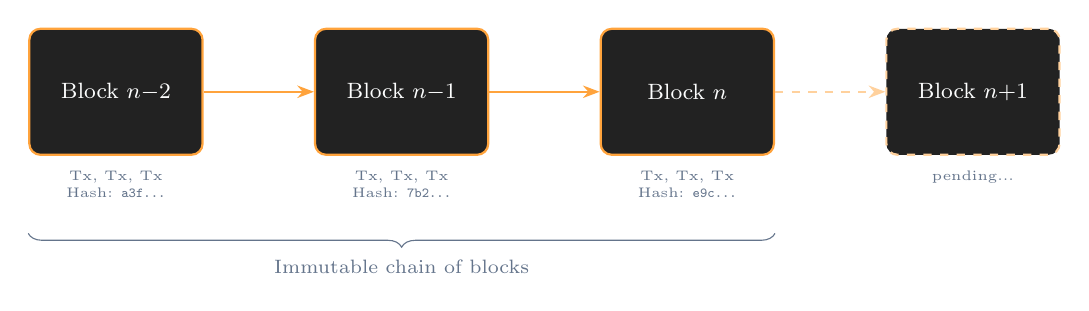
\begin{tikzpicture}[
      block/.style={
        rectangle, rounded corners=4pt,
        minimum width=2.2cm, minimum height=1.6cm,
        draw=ap3orange, thick, fill=ap3darkgray,
        font=\footnotesize\color{ap3cream}
      },
      arrow/.style={-{Stealth[length=6pt]}, thick, ap3orange},
      label/.style={font=\tiny\color{ap3slate}, align=center}
    ]
      % Blocks
      \node[block] (b1) {Block $n{-}2$};
      \node[block, right=1.4cm of b1] (b2) {Block $n{-}1$};
      \node[block, right=1.4cm of b2] (b3) {Block $n$};
      \node[block, right=1.4cm of b3, draw=ap3orange!50, dashed] (b4) {Block $n{+}1$};

      % Chain arrows
      \draw[arrow] (b1) -- (b2);
      \draw[arrow] (b2) -- (b3);
      \draw[arrow, ap3orange!50, dashed] (b3) -- (b4);

      % Block contents
      \node[label, below=2pt of b1] {Tx, Tx, Tx\\Hash: \texttt{a3f...}};
      \node[label, below=2pt of b2] {Tx, Tx, Tx\\Hash: \texttt{7b2...}};
      \node[label, below=2pt of b3] {Tx, Tx, Tx\\Hash: \texttt{e9c...}};
      \node[label, below=2pt of b4] {pending...};

      % Chain label
      \draw[decorate, decoration={brace, amplitude=5pt, mirror}, ap3slate]
        ([yshift=-28pt]b1.south west) -- ([yshift=-28pt]b3.south east)
        node[midway, below=6pt, font=\scriptsize\color{ap3slate}] {Immutable chain of blocks};
    \end{tikzpicture}
  \end{center}

  \note{
    Transactions are bundled into blocks, and each block stores the hash of the previous one.
    If someone tampers with an old block, every subsequent hash breaks and the network rejects it.
    Thousands of nodes worldwide hold identical copies of this chain.
    Users pay gas fees in ETH to compensate validators and prevent spam.
  }
\end{frame}

% ============================================================================
% SLIDE - Anatomy of an ETH Transfer
% ============================================================================
\begin{frame}{Anatomy of an ETH Transfer}
  \begin{itemize}
    \setlength{\itemsep}{12pt}
    \item A sender signs a transaction with their \textbf{private key},\\
          specifying recipient, amount, and gas limit
    \item The transaction is broadcast to the network, picked up\\
          by a validator, and included in the next block
    \item Sender's balance decreases, recipient's balance increases -\\
          all \textbf{atomic}: it either fully succeeds or fully reverts
  \end{itemize}

  \vspace{6pt}
  \begin{center}
    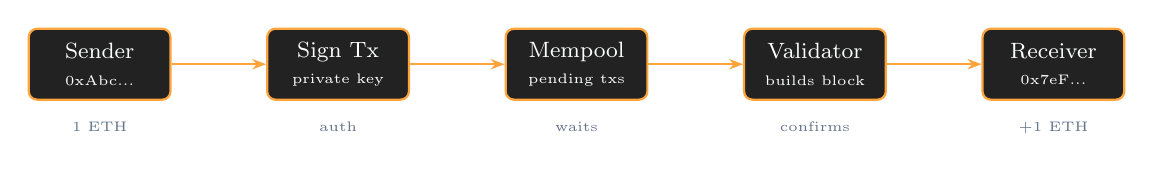
\begin{tikzpicture}[
      box/.style={
        rectangle, rounded corners=3pt,
        minimum width=1.8cm, minimum height=0.9cm,
        draw=ap3orange, thick, fill=ap3darkgray,
        font=\footnotesize\color{ap3cream}, align=center
      },
      arrow/.style={-{Stealth[length=5pt]}, thick, ap3orange},
      label/.style={font=\tiny\color{ap3slate}, align=center}
    ]
      \node[box] (sender) {Sender\\{\tiny 0xAbc...}};
      \node[box, right=1.2cm of sender] (sign) {Sign Tx\\{\tiny private key}};
      \node[box, right=1.2cm of sign] (mempool) {Mempool\\{\tiny pending txs}};
      \node[box, right=1.2cm of mempool] (validator) {Validator\\{\tiny builds block}};
      \node[box, right=1.2cm of validator] (receiver) {Receiver\\{\tiny 0x7eF...}};

      \draw[arrow] (sender) -- (sign);
      \draw[arrow] (sign) -- (mempool);
      \draw[arrow] (mempool) -- (validator);
      \draw[arrow] (validator) -- (receiver);

      \node[label, below=4pt of sender] {1 ETH};
      \node[label, below=4pt of sign] {auth};
      \node[label, below=4pt of mempool] {waits};
      \node[label, below=4pt of validator] {confirms};
      \node[label, below=4pt of receiver] {+1 ETH};
    \end{tikzpicture}
  \end{center}

  \note{
    The sender signs the transaction with their private key, proving ownership without revealing it.
    The signed transaction lands in the mempool, then a validator picks it up and includes it in a block.
    The operation is atomic: either the full transfer happens, or nothing happens.
    A simple ETH transfer costs 21,000 gas units, the cheapest operation on Ethereum.
  }
\end{frame}

% ============================================================================
% SLIDE 5 - Ethereum Key Concepts
% ============================================================================
\begin{frame}{Ethereum Key Concepts}
  \begin{itemize}
    \setlength{\itemsep}{12pt}
    \item \textcolor{ap3orange}{Ether (ETH)} - the native currency; used to pay gas fees
    \item \textcolor{ap3orange}{EVM} - the Ethereum Virtual Machine; executes code\\
          identically on every node (like a shared global CPU)
    \item \textcolor{ap3orange}{Proof of Stake} - validators lock ETH as collateral;\\
          dishonest behavior = funds get slashed
  \end{itemize}

  \note{
    ETH serves as both a currency and the fuel for the network.
    The EVM is what makes Ethereum programmable: every node runs the same virtual machine,
    so any computation always produces the same result everywhere. Like a shared Google Sheet.
    Proof of Stake replaced mining in 2022. Validators stake 32 ETH; cheating means slashing.
  }
\end{frame}

% ============================================================================
% SLIDE - The Merge: From PoW to PoS
% ============================================================================
\begin{frame}{The Merge: From PoW to PoS}
  \begin{itemize}
    \setlength{\itemsep}{12pt}
    \item \textcolor{ap3orange}{Proof of Work} (2015-2022): miners solve complex puzzles\\
          to validate blocks, consuming massive amounts of energy
    \item \textcolor{ap3orange}{The Merge} (Sept. 2022): Ethereum switched to\\
          \textbf{Proof of Stake}, reducing energy use by \textbf{99.95\%}
    \item \textcolor{ap3orange}{Proof of Stake}: validators lock 32 ETH as collateral;\\
          if they cheat, their stake gets \textbf{slashed} (destroyed)
  \end{itemize}

  \vspace{6pt}
  \begin{center}
    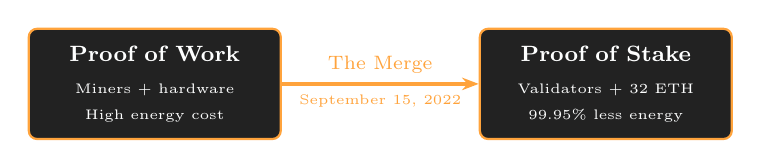
\begin{tikzpicture}[
      box/.style={
        rectangle, rounded corners=3pt,
        minimum width=3.2cm, minimum height=1.4cm,
        draw=ap3orange, thick, fill=ap3darkgray,
        font=\footnotesize\color{ap3cream}, align=center
      },
      arrow/.style={-{Stealth[length=6pt]}, very thick, ap3orange},
      label/.style={font=\tiny\color{ap3slate}, align=center}
    ]
      \node[box] (pow) {
        \textbf{Proof of Work}\\[2pt]
        {\tiny Miners + hardware}\\
        {\tiny High energy cost}
      };
      \node[box, right=2.5cm of pow] (pos) {
        \textbf{Proof of Stake}\\[2pt]
        {\tiny Validators + 32 ETH}\\
        {\tiny 99.95\% less energy}
      };

      \draw[arrow] (pow) -- node[above, font=\scriptsize\color{ap3orange}] {The Merge} 
                             node[below, label] {September 15, 2022} (pos);
    \end{tikzpicture}
  \end{center}

  \note{
    From 2015 to 2022, Ethereum used Proof of Work: miners competed with hardware to solve puzzles,
    consuming as much electricity as a small country. On September 15, 2022, The Merge switched
    Ethereum to Proof of Stake, cutting energy use by 99.95\%. Validators now lock 32 ETH as a deposit.
    If they cheat or go offline, the protocol slashes their stake. Same security, aligned incentives.
  }
\end{frame}

% ============================================================================
% SECTION 2: SMART CONTRACTS
% ============================================================================
\section{Smart Contracts \& Oracles}

% ============================================================================
% SLIDE 6 - What Are Smart Contracts?
% ============================================================================
\begin{frame}{What Are Smart Contracts?}
  \begin{itemize}
    \setlength{\itemsep}{12pt}
    \item Programs stored on the blockchain that \textbf{execute automatically}\\
          when predefined conditions are met
    \item Analogy: a \textcolor{ap3orange}{vending machine} - insert coin, get product;\\
          no cashier needed, rules are hardcoded
    \item Once deployed, the code is \textbf{immutable} and \textbf{transparent}  - \\
          anyone can read and verify it
  \end{itemize}

  \note{
    A smart contract is code that lives on the blockchain and self-executes when conditions are met.
    The vending machine analogy works well: insert coin, get product, no negotiation possible.
    Once deployed, the code is immutable. This enables trustless execution,
    but it also means bugs are permanent unless the contract has upgrade mechanisms.
  }
\end{frame}

% ============================================================================
% SLIDE 7 - Smart Contract Execution Flow
% ============================================================================
\begin{frame}{How Smart Contracts Execute}
  \begin{itemize}
    \setlength{\itemsep}{10pt}
    \item A user sends a \textbf{transaction} that triggers the contract
    \item The EVM executes the code; \textbf{all nodes verify} the result
    \item The new state is written permanently to the blockchain
  \end{itemize}

  \vspace{4pt}
  \begin{center}
    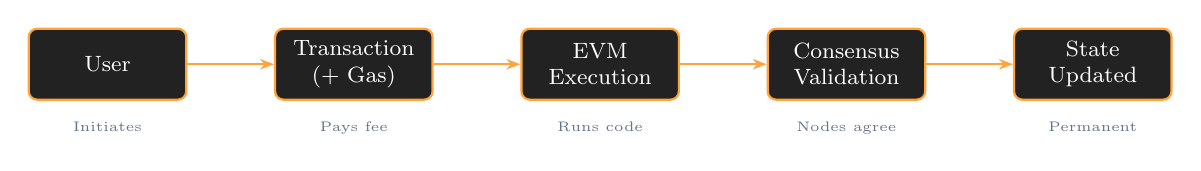
\begin{tikzpicture}[
      box/.style={
        rectangle, rounded corners=3pt,
        minimum width=2cm, minimum height=0.9cm,
        draw=ap3orange, thick, fill=ap3darkgray,
        font=\footnotesize\color{ap3cream}, align=center
      },
      arrow/.style={-{Stealth[length=5pt]}, thick, ap3orange},
      note/.style={font=\tiny\color{ap3slate}, align=center}
    ]
      % Flow nodes
      \node[box] (user) {User};
      \node[box, right=1.1cm of user] (tx) {Transaction\\(+ Gas)};
      \node[box, right=1.1cm of tx] (evm) {EVM\\Execution};
      \node[box, right=1.1cm of evm] (valid) {Consensus\\Validation};
      \node[box, right=1.1cm of valid] (state) {State\\Updated};

      % Arrows
      \draw[arrow] (user) -- (tx);
      \draw[arrow] (tx) -- (evm);
      \draw[arrow] (evm) -- (valid);
      \draw[arrow] (valid) -- (state);

      % Labels below
      \node[note, below=4pt of user] {Initiates};
      \node[note, below=4pt of tx] {Pays fee};
      \node[note, below=4pt of evm] {Runs code};
      \node[note, below=4pt of valid] {Nodes agree};
      \node[note, below=4pt of state] {Permanent};
    \end{tikzpicture}
  \end{center}

  \note{
    A user sends a transaction with gas to trigger the contract. The EVM runs the code,
    and all validators independently compute the same result. Once consensus is reached,
    the new state is written permanently on-chain. The whole process takes about 12 seconds.
    No single party controls the outcome; the code does.
  }
\end{frame}

% ============================================================================
% SLIDE - Upgradability & The Proxy Pattern
% ============================================================================
\begin{frame}{Upgradability \& The Proxy Pattern}
  \begin{itemize}
    \setlength{\itemsep}{12pt}
    \item Smart contracts are \textbf{immutable by default} -\\
          once deployed, the code can never be changed
    \item Problem: what if there's a bug, or the protocol needs to evolve?
    \item Solution: the \textcolor{ap3orange}{proxy pattern} - users interact with a\\
          fixed proxy that \textbf{delegates calls} to a replaceable logic contract
  \end{itemize}

  \vspace{6pt}
  \begin{center}
    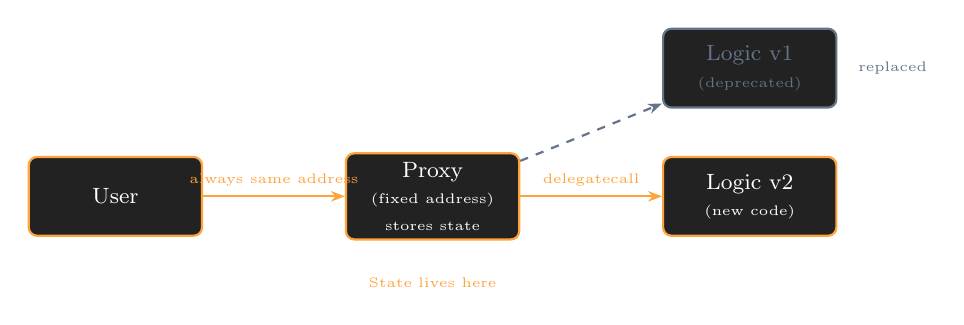
\begin{tikzpicture}[
      box/.style={
        rectangle, rounded corners=3pt,
        minimum width=2.2cm, minimum height=1cm,
        draw=ap3orange, thick, fill=ap3darkgray,
        font=\footnotesize\color{ap3cream}, align=center
      },
      oldbox/.style={
        rectangle, rounded corners=3pt,
        minimum width=2.2cm, minimum height=1cm,
        draw=ap3slate, thick, fill=ap3darkgray,
        font=\footnotesize\color{ap3slate}, align=center
      },
      arrow/.style={-{Stealth[length=5pt]}, thick, ap3orange},
      darrow/.style={-{Stealth[length=5pt]}, thick, ap3slate, dashed},
      label/.style={font=\tiny\color{ap3slate}}
    ]
      \node[box] (user) {User};
      \node[box, right=1.8cm of user] (proxy) {Proxy\\{\tiny (fixed address)}\\{\tiny stores state}};
      \node[box, right=1.8cm of proxy] (v2) {Logic v2\\{\tiny (new code)}};
      \node[oldbox, above=0.6cm of v2] (v1) {Logic v1\\{\tiny (deprecated)}};

      \draw[arrow] (user) -- node[above, label] {always same address} (proxy);
      \draw[arrow] (proxy) -- node[above, label] {delegatecall} (v2);
      \draw[darrow] (proxy) -- node[left, label] {} (v1);

      \node[font=\tiny\color{ap3orange}, below=10pt of proxy] {State lives here};
      \node[font=\tiny\color{ap3slate}, right=4pt of v1] {replaced};
    \end{tikzpicture}
  \end{center}

  \note{
    The proxy contract holds all the state and keeps a fixed address. It delegates execution
    to a separate logic contract via delegatecall. To upgrade, you deploy new logic and update the pointer.
    Most major DeFi protocols use this: Aave, Compound, Uniswap governance.
    The tradeoff is a trust assumption on whoever controls the upgrade key, often mitigated by multisig or DAO.
  }
\end{frame}

% ============================================================================
% SLIDE 8 - The Oracle Problem
% ============================================================================
\begin{frame}{The Oracle Problem}
  \begin{itemize}
    \setlength{\itemsep}{12pt}
    \item Blockchains are \textbf{isolated} - they can't access external data\\
          (prices, weather, sports scores) on their own
    \item \textcolor{ap3orange}{Oracles} are trusted data bridges between the\\
          real world and smart contracts
    \item Example: Chainlink aggregates price feeds from multiple\\
          sources to prevent manipulation
  \end{itemize}

  \vspace{2pt}
  \begin{center}
    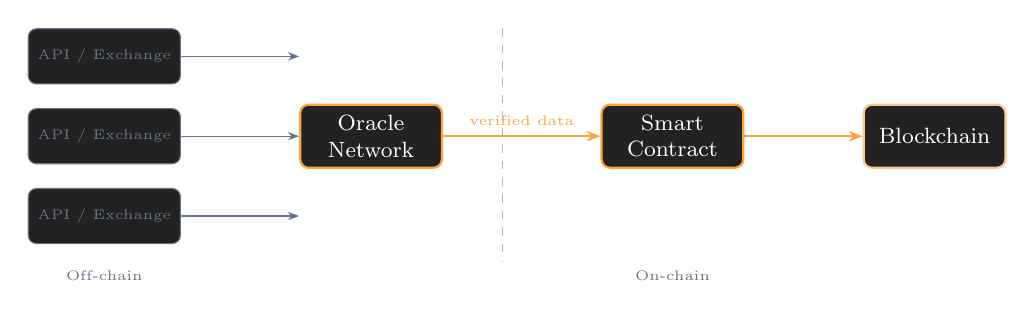
\begin{tikzpicture}[
      box/.style={
        rectangle, rounded corners=3pt,
        minimum width=1.8cm, minimum height=0.8cm,
        draw=ap3orange, thick, fill=ap3darkgray,
        font=\footnotesize\color{ap3cream}, align=center
      },
      src/.style={
        rectangle, rounded corners=3pt,
        minimum width=1.6cm, minimum height=0.7cm,
        draw=ap3slate, fill=ap3darkgray,
        font=\tiny\color{ap3slate}, align=center
      },
      arrow/.style={-{Stealth[length=5pt]}, thick, ap3orange},
      darrow/.style={-{Stealth[length=4pt]}, ap3slate}
    ]
      % Data sources
      \node[src] (api1) {API / Exchange};
      \node[src, below=0.3cm of api1] (api2) {API / Exchange};
      \node[src, below=0.3cm of api2] (api3) {API / Exchange};

      % Oracle network
      \node[box, right=1.5cm of api2] (oracle) {Oracle\\Network};

      % Smart contract
      \node[box, right=2cm of oracle] (sc) {Smart\\Contract};

      % Blockchain
      \node[box, right=1.5cm of sc, draw=ap3orange!60] (chain) {Blockchain};

      % Arrows
      \draw[darrow] (api1.east) -- (oracle.west |- api1.east);
      \draw[darrow] (api2.east) -- (oracle.west);
      \draw[darrow] (api3.east) -- (oracle.west |- api3.east);

      \draw[arrow] (oracle) -- node[above, font=\tiny\color{ap3slate}] {verified data} (sc);
      \draw[arrow] (sc) -- (chain);

      % Labels
      \node[font=\tiny\color{ap3slate}, below=6pt of api2 |- api3.south] {Off-chain};
      \node[font=\tiny\color{ap3slate}, below=6pt of sc |- api3.south] {On-chain};

      % Divider
      \draw[dashed, ap3slate!50] ([xshift=0.75cm]oracle.east |- api1.north) -- 
                                   ([xshift=0.75cm, yshift=-6pt]oracle.east |- api3.south);
    \end{tikzpicture}
  \end{center}

  \note{
    Smart contracts are blind: they can only see data that's already on-chain.
    Oracles bridge this gap by fetching real-world data (prices, events), aggregating it
    from multiple sources, and delivering it on-chain in a tamper-resistant way.
    Chainlink is the dominant provider, using decentralized node operators with economic incentives.
    Without oracles, DeFi as we know it simply couldn't exist.
  }
\end{frame}

% ============================================================================
% SECTION 3: STABLECOINS
% ============================================================================
\section{The Invention of Stablecoins}

% ============================================================================
% SLIDE 9 - Why Stablecoins?
% ============================================================================
\begin{frame}{Why Stablecoins?}
  \begin{itemize}
    \setlength{\itemsep}{12pt}
    \item Crypto is volatile - ETH can swing \textbf{10\%+ in a day};\\
          this makes it impractical for payments or savings
    \item Stablecoins are tokens \textbf{pegged to a stable asset}\\
          (usually \$1 USD), combining crypto rails with price stability
    \item They are now the \textcolor{ap3orange}{most used tokens on-chain}  - \\
          over \$150B+ in circulation (2025)
  \end{itemize}

  \note{
    ETH can swing 10\%+ in a day, making it impractical for payments or savings.
    Stablecoins solve this by combining the speed of crypto with dollar stability.
    Over \$150B in circulation as of 2025, with USDT and USDC leading the market.
    Often called crypto's ``killer app'' because they make the tech genuinely usable.
  }
\end{frame}

% ============================================================================
% SLIDE 10 - Types of Stablecoins
% ============================================================================
\begin{frame}{Types of Stablecoins}
  \begin{columns}[T]
    \begin{column}{0.32\textwidth}
      \textcolor{ap3orange}{\textbf{Fiat-Backed}}\\[6pt]
      \textcolor{ap3light}{\small
        Backed 1:1 by USD\\
        in bank accounts.\\[4pt]
        \textcolor{ap3slate}{\footnotesize Examples:\\USDC, USDT}
      }
    \end{column}
    \begin{column}{0.32\textwidth}
      \textcolor{ap3orange}{\textbf{Crypto-Backed}}\\[6pt]
      \textcolor{ap3light}{\small
        Over-collateralized\\
        by crypto assets.\\[4pt]
        \textcolor{ap3slate}{\footnotesize Examples:\\DAI, LUSD}
      }
    \end{column}
    \begin{column}{0.32\textwidth}
      \textcolor{ap3orange}{\textbf{Algorithmic}}\\[6pt]
      \textcolor{ap3light}{\small
        Use mint/burn\\
        mechanisms to\\
        maintain the peg.\\[4pt]
        \textcolor{ap3slate}{\footnotesize Examples:\\FRAX, USDe}
      }
    \end{column}
  \end{columns}

  \note{
    Fiat-backed is the simplest: one token equals one dollar held in a bank account (USDC, USDT).
    Crypto-backed uses on-chain collateral with over-collateralization (DAI requires 150\%).
    Algorithmic stablecoins use mint/burn mechanics and are the riskiest.
    The TerraUST collapse in 2022 wiped out \$40B overnight, showing the danger of bad design.
  }
\end{frame}

% ============================================================================
% SLIDE 11 - Stablecoin Collateral Model
% ============================================================================
\begin{frame}{How Fiat-Backed Stablecoins Work}
  \begin{itemize}
    \setlength{\itemsep}{10pt}
    \item Users deposit USD $\rightarrow$ issuer mints equivalent tokens
    \item Reserves are held in \textbf{regulated bank accounts} \& T-bills
    \item Redemption: burn tokens $\rightarrow$ receive USD back
  \end{itemize}

  \vspace{4pt}
  \begin{center}
    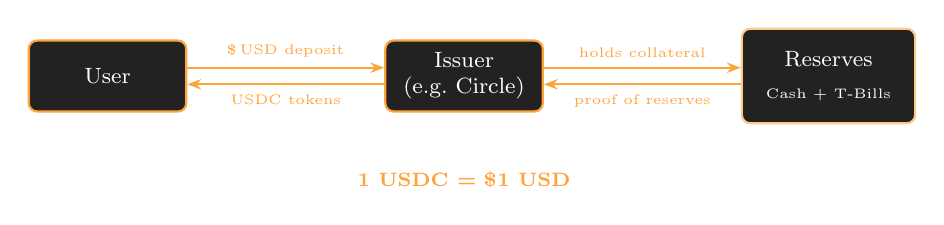
\begin{tikzpicture}[
      box/.style={
        rectangle, rounded corners=3pt,
        minimum width=2cm, minimum height=0.9cm,
        draw=ap3orange, thick, fill=ap3darkgray,
        font=\footnotesize\color{ap3cream}, align=center
      },
      reserve/.style={
        rectangle, rounded corners=3pt,
        minimum width=2.2cm, minimum height=1.2cm,
        draw=ap3orange!60, thick, fill=ap3darkgray,
        font=\footnotesize\color{ap3cream}, align=center
      },
      arrow/.style={-{Stealth[length=5pt]}, thick, ap3orange},
      label/.style={font=\tiny\color{ap3slate}}
    ]
      % User
      \node[box] (user) {User};

      % Issuer
      \node[box, right=2.5cm of user] (issuer) {Issuer\\(e.g.\ Circle)};

      % Reserve
      \node[reserve, right=2.5cm of issuer] (reserve) {Reserves\\[2pt]\tiny Cash + T-Bills};

      % Arrows
      \draw[arrow] ([yshift=3pt]user.east) -- node[above, label] {\$\,USD deposit} ([yshift=3pt]issuer.west);
      \draw[arrow] ([yshift=-3pt]issuer.west) -- node[below, label] {USDC tokens} ([yshift=-3pt]user.east);

      \draw[arrow] ([yshift=3pt]issuer.east) -- node[above, label] {holds collateral} ([yshift=3pt]reserve.west);
      \draw[arrow] ([yshift=-3pt]reserve.west) -- node[below, label] {proof of reserves} ([yshift=-3pt]issuer.east);

      % 1:1 label
      \node[font=\scriptsize\bfseries\color{ap3orange}, below=18pt of issuer] {1 USDC = \$1 USD};
    \end{tikzpicture}
  \end{center}

  \note{
    A user sends dollars to Circle, which mints the equivalent USDC tokens on-chain.
    The reserves are held in regulated bank accounts and short-term T-bills.
    To redeem, you burn your USDC and Circle wires back the dollars.
    The key trust assumption: you trust that Circle actually holds the reserves.
    They publish monthly attestation reports from Deloitte to prove it.
  }
\end{frame}

% ============================================================================
% SLIDE 12 - Crypto-Backed Stablecoins (MakerDAO Example)
% ============================================================================
\begin{frame}{Crypto-Backed: The MakerDAO Model}
  \begin{itemize}
    \setlength{\itemsep}{10pt}
    \item Deposit \$150 of ETH $\rightarrow$ borrow up to \$100 of DAI\\
          (\textcolor{ap3orange}{150\% collateral ratio} absorbs price drops)
    \item If collateral value drops below threshold $\rightarrow$\\
          \textbf{automatic liquidation} protects the system
    \item Fully on-chain, transparent, no bank required
  \end{itemize}

  \vspace{4pt}
  \begin{center}
    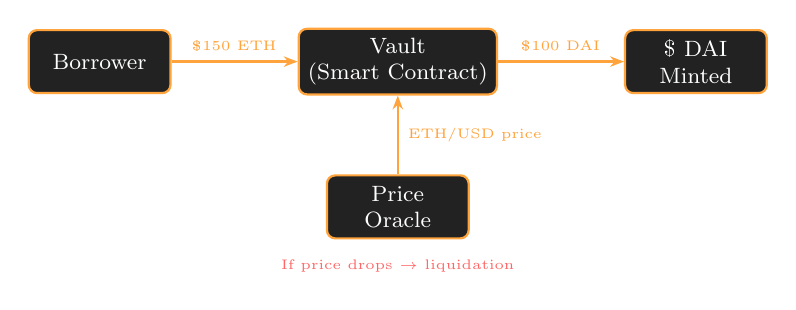
\begin{tikzpicture}[
      box/.style={
        rectangle, rounded corners=3pt,
        minimum width=1.8cm, minimum height=0.8cm,
        draw=ap3orange, thick, fill=ap3darkgray,
        font=\footnotesize\color{ap3cream}, align=center
      },
      arrow/.style={-{Stealth[length=5pt]}, thick, ap3orange},
      redarrow/.style={-{Stealth[length=5pt]}, thick, red!60},
      label/.style={font=\tiny\color{ap3slate}}
    ]
      \node[box] (user) {Borrower};
      \node[box, right=1.6cm of user] (vault) {Vault\\(Smart Contract)};
      \node[box, right=1.6cm of vault] (dai) {\$ DAI\\Minted};
      \node[box, below=1cm of vault] (oracle) {Price\\Oracle};

      \draw[arrow] (user) -- node[above, label] {\$150 ETH} (vault);
      \draw[arrow] (vault) -- node[above, label] {\$100 DAI} (dai);
      \draw[arrow] (oracle) -- node[right, label] {ETH/USD price} (vault);

      % Liquidation path
      \node[font=\tiny\color{red!60}, below=4pt of oracle] {If price drops $\rightarrow$ liquidation};
    \end{tikzpicture}
  \end{center}

  \note{
    You lock ETH into a Vault smart contract and can mint DAI up to 66\% of your collateral value.
    The 150\% ratio creates a buffer that absorbs price drops. If the collateral falls below
    the threshold, the smart contract automatically liquidates it to protect the system.
    Price oracles feed the ETH/USD rate. The entire process is trustless, no human decision.
  }
\end{frame}

% ============================================================================
% SLIDE 13 - Stablecoins: Real-World Impact
% ============================================================================
\begin{frame}{Stablecoins: Real-World Impact}
  \begin{itemize}
    \setlength{\itemsep}{12pt}
    \item \textcolor{ap3orange}{Payments} - instant, borderless transfers at near-zero cost;\\
          already adopted in emerging markets for remittances
    \item \textcolor{ap3orange}{DeFi backbone} - stablecoins are the unit of account\\
          for lending, trading, and yield strategies on-chain
    \item \textcolor{ap3orange}{Institutional adoption} - major banks and fintechs\\
          are integrating stablecoin settlement (PayPal, Visa, Stripe)
  \end{itemize}

  \note{
    In emerging markets like Argentina or Nigeria, stablecoins serve as a digital dollar savings account.
    In DeFi, they're the base pair for trading, lending, and yield strategies.
    On the institutional side, PayPal launched PYUSD, Visa settles in USDC, and Stripe acquired Bridge.
    Regulation is catching up with the EU's MiCA framework and proposed US legislation.
  }
\end{frame}

% ============================================================================
% SLIDE 14 - Key Takeaways
% ============================================================================
\begin{frame}{Key Takeaways}
  \begin{itemize}
    \setlength{\itemsep}{14pt}
    \item \textcolor{ap3orange}{Ethereum} turned blockchains from ledgers into\\
          \textbf{programmable platforms} - enabling an entire ecosystem
    \item \textcolor{ap3orange}{Smart contracts + oracles} automate trust and\\
          connect on-chain logic to real-world data
    \item \textcolor{ap3orange}{Stablecoins} bridge crypto volatility and real-world\\
          usability - now a \textbf{\$150B+} market and growing
  \end{itemize}

  \vspace{12pt}
  \begin{center}
    \textcolor{ap3slate}{\small These three innovations form the foundation of\\
    modern decentralized finance (DeFi).}
  \end{center}

  \note{
    Ethereum turned blockchains into programmable platforms, enabling an entire ecosystem.
    Smart contracts paired with oracles automate trust and connect on-chain logic to real-world data.
    Stablecoins solved the volatility problem and made crypto genuinely useful for everyday finance.
    Together, these three pillars form the foundation of modern DeFi.
  }
\end{frame}

% ============================================================================
% SLIDE 15 - Thank You / Q&A
% ============================================================================
\begin{frame}[plain]
  \vfill
  \begin{center}
    {\usebeamerfont{title}\textcolor{ap3orange}{Thank You}}\\[16pt]
    \textcolor{ap3orange}{\rule{0.2\textwidth}{1.5pt}}\\[16pt]
    {\large\textcolor{ap3cream}{Questions \& Discussion}}\\[24pt]
    \textcolor{ap3slate}{\small
      \href{https://ap3labs.com}{ap3labs.com}\quad$\cdot$\quad
      \href{https://x.com/alexis\_ap3labs}{@alexis\_ap3labs}\quad$\cdot$\quad
      \href{https://github.com/alexis-ap3labs}{github/alexis-ap3labs}
    }
  \end{center}
  \vfill

  \note{
    Thank you for your attention. The floor is open for questions.
    Happy to dive deeper into any of the topics we covered.
    Contact details are on screen.
  }
\end{frame}

\end{document}
